\begin{center}
	\Huge
	Ekstrema
\end{center}



\section*{Ekstrema}
\stepcounter{section}

 Vi kan se både en vandret vendetangent samt to ekstrema på Figur \ref{fig:ekstremavende}.


\begin{figure}[H]
	\centering
	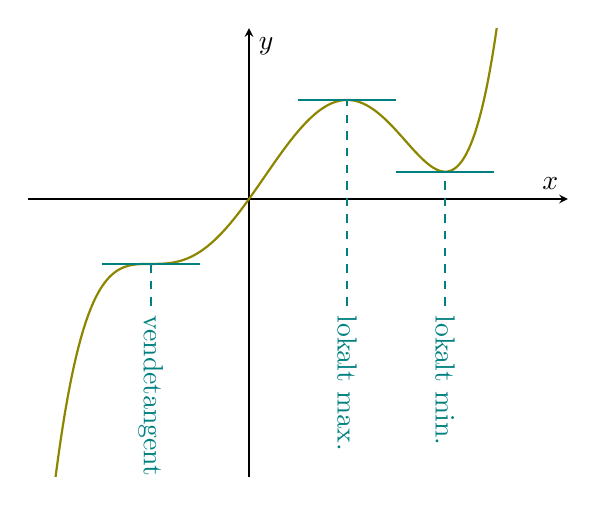
\begin{tikzpicture}
	\begin{axis}[
	axis lines = center, 
	xmin = -4.5, xmax = 6.5,
	ymin = -130, ymax = 80,
	xlabel = $x$, ylabel = $y$, 
	ticks = none,
	]
		\addplot[color = olive, thick, domain = -5:7, samples = 400] 
		{1/5*x^5-1/2*x^4-4*x^3+4*x^2+32*x };
		\node[color = teal, anchor = west, rotate = -90] at (axis cs: -2,-50) {vendetangent};
		\draw[color = teal, dashed, thick] (axis cs: -2,-50) -- (axis cs:-2,-152/5); 
		\node[color = teal, anchor = west, rotate = -90] at (axis cs: 2,-50) {lokalt max.};
		\draw[color = teal, dashed, thick] (axis cs: 2,-50) -- (axis cs:2,232/5); 
		\node[color = teal, anchor = west, rotate = -90] at (axis cs: 4,-50) {lokalt min.};
		\draw[color = teal, dashed, thick] (axis cs: 4,-50) -- (axis cs: 4,64/5); 
		\draw[color = teal, thick] (axis cs: -3,-152/5) -- (axis cs: -1,-152/5); 
		\draw[color = teal, thick] (axis cs: 1,232/5) -- (axis cs: 3,232/5); 
		\draw[color = teal, thick] (axis cs: 3,64/5) -- (axis cs: 5,64/5); 
	\end{axis}
	\end{tikzpicture}
	\caption{Forskellige ekstrema for en funktion samt vandrette tangenter}
	\label{fig:ekstremavende}
\end{figure}


Lad os som sidst betragte et eksempel.

\begin{exa}
	Lad $f$ være givet ved
	\begin{align*}
		f(x) = x^3-6x^2+5.
	\end{align*}
	Vi ønsker at bestemme ekstrema for $f$. Vi differentierer derfor først $f$.
	\begin{align*}
		f'(x) = 3x^2-12x = 3x(x-4).
	\end{align*}
	Dette sættes nu lig $0$, og vi får
	\begin{align*}
		3x(x-4) = 0, 
	\end{align*}
	og ved hjælp af nulreglen ved vi, at $x=0$ eller $x = 4$. Vi bestemmer nu de tilhørende $y$-værdier og vi får
	\begin{align*}
		f(0) = 5
	\end{align*}
	og 
	\begin{align*}
		f(4) &= 4^3 - 6\cdot 4^2+5\\
		&= 64-96+5\\
		&= -27.
	\end{align*}
	Vi har derfor en vandret tangent i $P(0,5)$ og $Q(4,-27)$. For at bestemme, om det er et ekstremumspunkt, så tegner vi grafen. Denne kan ses af Figur \ref{fig:ekstrema}
	\begin{figure}[H]
		\centering
		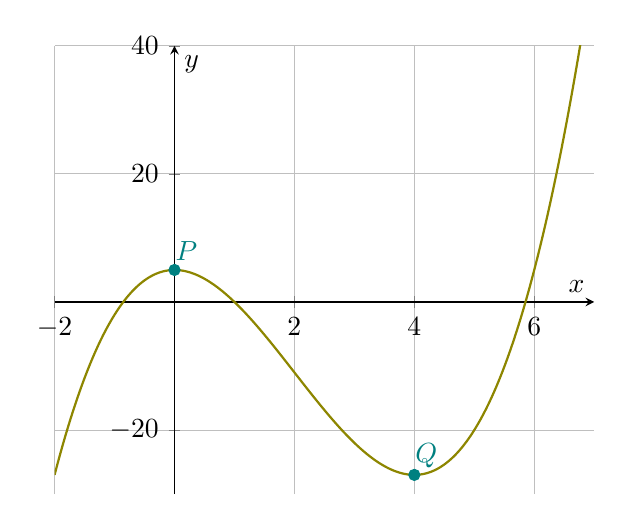
\begin{tikzpicture}
			\begin{axis}[axis lines = middle,
			xmin = -2, xmax = 7,
			ymin = -30, ymax = 40,
			xlabel = $x$, 
			ylabel = $y$,
			grid = both]
				\addplot[color = olive, samples = 200, domain = -2:7, thick] {x^3-6*x^2+5};
				\filldraw[color = teal] (axis cs:0,5) circle (2pt);
				\filldraw[color = teal] (axis cs:4,-27) circle (2pt);
				\node[color = teal] at (axis cs: 0.2,8) {$P$};
				\node[color = teal] at (axis cs: 4.2,-24) {$Q$};
			\end{axis}
		\end{tikzpicture}
		\caption{Graf for funktionen $f$.}
		\label{fig:ekstrema}
	\end{figure}
\end{exa}
Af Figur \ref{fig:ekstrema} kan vi se, at punkterne $P$ og $Q$ er ekstremumspunkter. $P$ er et \textit{lokalt maksimum} og $Q$ er et \textit{lokalt minimum}. Vi kan også se, at $f$ ikke har nogle 
\textit{globale ekstrema}.

Vi inkluderer for en god ordens skyld tabellen med differentialkvotienter.

\begin{table}[H]
	\centering
	\rowcolors{1}{white}{teal!30}
	\begin{tabular}{cc}
		$f(x)$ & $f'(x)$ \\
		$k$ & $0$ \\
		$x$ & $1$ \\
		$ax + b$  & $a$ \\
		$x^2$ & $2x$ \\
		$x^a$ & $ax^{a-1} $ \\
		$\sqrt{x}$ & $\frac{1}{2\sqrt{x}}$ \\
		$\frac{1}{x}$ & $-\frac{1}{x^2}$ \\
		$\ln(x)$ & $\frac{1}{x}$ \\
	 	$e^x$ & $e^x$ \\
	 	$\cos(x)$ & $-\sin(x)$ \\
	 	$\sin(x)$ & $\cos(x)$ \\
	\end{tabular}
	\caption{Udvalgte afledede funktioner}
	\label{tab:afledt}
\end{table}





\subsection*{Opgave 1 (Med hjælpemidler)}

Bestem ekstremumspunkter for følgende funktioner. Løs først ligningen $f'(x)=0$ og tegn derefter grafen for funktionen.  Afgør til sidst, om der er tale om globale maksimum/minimum eller lokale maksimum/minimum.

\begin{align*}
	&1) \ f(x) =  2\ln(x) - x^3    &&2) \ f(x) =   2x^5 - 4x^4 + 3x^3 - 2x^2    \\
	&3) \ f(x) = 5\sqrt(x) + 4x^3 - x^4    &&4) \ f(x) = \cos(x)^2 - \sin(x^2), \ 0 \leq x \leq 4    \\
\end{align*}


\subsection*{Opgave 2}
Vis, at et andengradspolynomium $p$ givet ved
\begin{align*}
	p(x) = ax^2 + bx + c
\end{align*}
har ekstrema i punktet $P$ givet ved
\begin{align*}
	P\left(\frac{-b}{2a},\frac{-d}{4a}\right),
\end{align*}
hvor $d$ er diskriminanten for $p$. 

\subsection*{Opgave 3 (Med hjælpemidler)}
Et andengradspolynomium $p$ er givet ved
\begin{align}
		p(x) = 2x^2 + bx + 4.
\end{align}
\begin{enumerate}[label=\roman*)]
	\item Bestem tallet $b$, så toppunktet for $p$ ligger på $x$-aksen.
\end{enumerate}

\subsection*{Opgave 4 (Med hjælpemidler)}
To polynomier $p$ og $q$ er givet ved 
\begin{align*}
	p(x) = ax^3 - 5x^2 + 2x + d \quad \textnormal{og} \quad q(x) = x^2 + 2x + 1
\end{align*}
\begin{enumerate}[label=\roman*)]
	\item Bestem tallene $a$ og $d$, så $p$ og $q$ har ekstrema i samme punkt. 
\end{enumerate}

\subsection*{Opgave 5}
Man kan bruge de såkaldt \textit{dobbeltafledede} til at afgøre, om et ekstremum er et maksimum eller et minimum. Hvis $f''(x_0) > 0$, så er $x_0$ et minimum, og hvis $f''(x_0) < 0$, så er $x_0$ et maksimum. Hvis $f''(x_0) = 0$, så bliver man nødt til at bruge andre metoder til at afgøre typen af ekstremum. 

\begin{enumerate}[label = \roman*)]
	\item Find ekstrema for $f(x) = x^2 -2x + 1$ og afgør typen af ekstremum
	\item Find ekstrema for $f(x) = x^3 - 3x^2$ og afgør typen af ekstrema
	\item Find ekstrema for $f(x) = \ln(x) - 0.5x^2$ og afgør typen af ekstrema
\end{enumerate}

\subsection*{Opgave 6}
Brug de dobbeltafledede til at forklare betydningen af $a$ i et andengradspolynomium 
\begin{align*}
	p(x) = ax^2 + bx + c.
\end{align*}

\subsection*{Opgave 7}
Overvej, hvorfor det giver intuitiv god mening at $f''(x_0) < 0$ medfører et maksimum og vice versa. Tegn evt en tegning af et andengradspolynomium $p$, samt af $p'$ og $p''$.
